\documentclass[11pt]{article}

\usepackage{url}
\usepackage{multicol}
\usepackage[english]{babel}
\usepackage[margin=1in]{geometry}
\usepackage{graphicx}
\usepackage{subcaption}
\usepackage{enumitem}
\usepackage{amsmath}
\usepackage{amssymb}
\usepackage{wasysym}
\usepackage{color}
\usepackage{float}
\usepackage{nomencl}
\usepackage[title]{appendix}
\makenomenclature
\usepackage{pdfpages}
\usepackage{algorithm}
\usepackage{algpseudocode}
\usepackage{hyperref}
\hypersetup{
    colorlinks=true,
    linkcolor=blue,
    filecolor=magenta,      
    urlcolor=cyan,
    pdftitle={Overleaf Example},
    pdfpagemode=FullScreen,
    }
\title{16-745 Optimal Control Lecture 12}
\author{Reid Graves} 

\begin{document}
\maketitle

\section{Last Time}
\begin{itemize}
    \item Nonlinear Trajectory Optimization
    \item DDP/iLQR
\end{itemize}

\section{Today}
\begin{itemize}
    \item DDP details + extensions
    \item Constraints
\end{itemize}

\section{DDP recap}
\begin{itemize}
    \item Solve the unconstrained trajectory optimization problem:
    \begin{align*}
        \min_{x_{1:N},u_{1:N-1}}\quad J &= \sum_{k=1}^{N-1}l(x_k,u_k) + l_N(x_N)
        \\
        \quad s.t.\quad x_{k+1} &= f(x_k,u_k)
    \end{align*}
    \item Backward Pass: - taylor expand
    \begin{align*}
        V_k(x+\Delta x) &\approx V(x) + p_k^T\Delta x + \frac{1}{2}\Delta x^TP_k\Delta x
        \\
        \quad P_N &= \nabla^2 l_n(x), \quad p_N =\nabla l_N(x)
    \end{align*}
    Go backwards with Bellman backup:
    \begin{align*}
        V_{N-1}(x + \Delta x) &= \min_{\Delta u} S(x+\Delta x, u + \Delta u)
        \\
        \Rightarrow \Delta u_{k-1} &= -d_{k-1} - K_{n-1}\Delta x_{k-1} 
        \\
        P_{k-1} &= G_{xx} + K^T G_{uu}K - G_{xu}K - K^T G_{ux}
        \\
        p_{k-1} &= g_k - K^Tg_u + K^T G_{uu}d  - G_{xu}D
    \end{align*}
    \item Forward Rollout
    \begin{align*}
        \Delta J &= 0 
        \\
        x_k' &= x_1
        \\
        &for \quad k=1:N-1:
        \\
        &\quad u_k' = u-\alpha d_k - K_k(x_k'-k_k)
        \\
        &\quad x_{k+1}' = f(x_k', u_k')
        \\
        &\quad \Delta J \leftarrow \Delta J + \alpha g_{ux}d_k
        \\
        end
    \end{align*}
    \item Line search:
    \begin{align*}
        \alpha &=1 
        \\
        & do: \\
       &\quad x',u',\Delta J = rollout(x,u,d,K,\alpha)
       \\
       &\quad \alpha \leftarrow c\alpha
       \\
       &while \quad J(x',u') < J(x,u) - b\Delta J
       \\
       & x,u \leftarrow x',u'
    \end{align*}
\end{itemize}

\subsection{Examples}
\begin{itemize}
    \item Cartpole + acrobot swing up
    \item DDP can converge in fewer iterations but iLQR often wins in wall-clock time
    \item Problems are conconvex $\Rightarrow$ can land in different local optima depending on initial guess
\end{itemize}

\subsection{Regularization}
\begin{itemize}
    \item Just like standard Newton, $V(x)$ and/or $S(x,u)$ Hessians can become indefinite in backward pass
    \item Regularization is deffinitely necessary for DDP, often a good idea with iLQR as well.
    \item Many options for regularizing:
    \begin{itemize}
        \item Add a multiple of identity to $\nabla^2 S(x,u)$
        \item Regularize $P_k$ or $G_k$ as needed in the backward pass
        \item Regularize just $G_{uu} = \nabla_{uu}^2S(x,u)$ (this is the only matrix you have to invert):
        \begin{align*}
            d &= G_{uu}^{-1}g_u, \quad K = G_{uu}^{-1}G_{ux}
        \end{align*}
    \end{itemize}
    \item This last one is good fo iLQR but not DDP
    \item Regularization should not be required for iLQR but can be necessary due to floating point error.
\end{itemize}
\subsection{DDP notes}
\subsubsection{Pros}
\begin{itemize}
    \item Can be very fast (iterations + wall-clock)
    \item One of the most efficient methods due to exploitation of DP structure
    \item Always dynamically feasible due to forward rollout $\Rightarrow$ can always execute on robot
    \item Comes with TVLQR tracking controller for free $\Rightarrow$ 
\end{itemize}
\subsubsection{Cons}
\begin{itemize}
    \item Does not natively handle constraints
    \item Does not support infeasible initial guess for state trajectory due to forward rollout. Bad for ``maze" or ``bug-trap" problems
    \item Can suffer from numerical ill-conditioning on long trajectories
\end{itemize}

\section{Handling Constraints in DDP}
\begin{itemize}
    \item Many options depending on type of constraint
    \item Torque limits con be handled with a ``squashing function" e.g. $\tanh:$
    % insert figure here
    \begin{figure}[H]
        \centering
        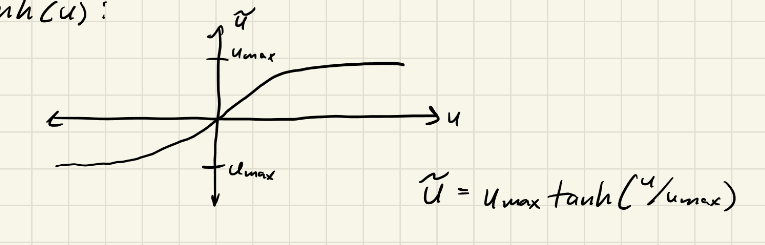
\includegraphics[width=0.9\linewidth]{lecture_12_1.png}
    \end{figure}
    \item Effective, but adds nonlinearity and may need more iterations
    \item Better option: solve box-constrained QP in the backward pass:
    \begin{align*}
        \Delta u &= \text{arg}\min_{\Delta u} S(x+\Delta x, u + \Delta u)
        \\
        &\quad s.t. \quad u_{min}\leq u+\Delta u \leq u_{max}
    \end{align*}
    \item State constraints are harder. Often penalties are added to cost function. Can cause ill-conditioning
    \item Better Option: Wrap entire DDP algorithm in an Augmented Lagrangian method
    \item Augmented Lagrangian method adds linear (multiplier) and quadratic (penalty) terms to the cost $\Rightarrow$ fits into DDP nicely
\end{itemize}




\end{document}
